\documentclass[11pt,british]{report}
\renewcommand{\rmdefault}{ptm}
\renewcommand{\familydefault}{\rmdefault}
%formatting packages
\usepackage[T1]{fontenc}
\usepackage[latin9]{inputenc}
\usepackage[a4paper]{geometry}
\geometry{verbose,tmargin=2.9cm,bmargin=2.9cm,lmargin=2.3cm,rmargin=2.3cm}
%\usepackage{fancyhdr}
%\pagestyle{fancy}
\setcounter{secnumdepth}{3}
\usepackage[british]{babel}
\usepackage{booktabs}
\usepackage{array,multirow}
\usepackage{subfig}
\usepackage[explicit]{titlesec}
\usepackage{adjustbox}
\usepackage{cite}
\usepackage{pdfpages}
\usepackage{standalone}
\usepackage[toc,page]{appendix}
\usepackage{listings}
\usepackage{setspace}
\usepackage{acro}
\usepackage{etoolbox}

%%maths
\usepackage{units}
\usepackage{siunitx}
\usepackage{amsmath}
\usepackage{amssymb}
\usepackage{mathrsfs}
%\usepackage{commath}
\usepackage{cancel}
\usepackage{gensymb}
\usepackage{esint}
\usepackage{mdsymbol}
%\usepackage{eurosym} 
%\usepackage{wasysym}

%%figures
\usepackage{graphicx}
\usepackage{esvect}
\usepackage{color}
\usepackage{xcolor}
\usepackage{float}
\usepackage{caption}
\usepackage{placeins}

%\usepackage{tikz}

\usepackage[
	unicode=true,pdfusetitle,
	bookmarks=true,bookmarksnumbered=false,bookmarksopen=false,
	breaklinks=true,pdfborder={0 0 0},backref=page,colorlinks=false
	]{hyperref}

\makeatletter
\lst@InstallKeywords k{attributes}{attributestyle}\slshape{attributestyle}{}ld
\makeatother
\makeatletter
\lst@InstallKeywords k{modules}{modulestyle}\slshape{modulestyle}{}ld
\makeatother

\lstdefinestyle{c-style}
{
	language=C,
	showstringspaces=false,
	breaklines=true,
	breakatwhitespace=true,
	numbers=none,
	tabsize=4,
	lineskip=-0.7ex,
	basicstyle=\footnotesize\selectfont\ttfamily,
	keywordstyle=\color{blue}\ttfamily,
	stringstyle=\color{red}\ttfamily,
	commentstyle=\color{vgreen}\ttfamily,
	morecomment=[l][\color{magenta}]{\#},
	morekeywords={uint8\_t, uint16\_t, uint32\_t, interrupt, int16\_t, UL, SPI\_t},
	moreattributes={DISPLAY\_CLIPPING\_THRESH, ADXL\_WRITE\_COMMAND,ADXL\_SS\_POS,SPI\_DATA\_READY,ADXL\_SS\_POS,SPI\_WRITE\_COMPLETE,VALUE\_1\_OFFSET,VALUE\_2\_OFFSET,NVIC\_ADXL\_BIT\_POS,ADXL\_DATA\_START,DISPLAY\_DIGITS\_PER\_VAR,DISPLAY\_MINUS,DISPLAY\_BLANK}, % etc...
	attributestyle = \bfseries\color{mymauve} % (for instance)
}

\lstdefinestyle{verilog-style}
{
	language=Verilog,
	basicstyle=\footnotesize\selectfont\ttfamily,
	%breakatwhitespace=true,
	breaklines=true,
	keywordstyle=\color{vblue}\ttfamily,
	identifierstyle=\color{black}\ttfamily,
	commentstyle=\color{vgreen}\ttfamily,
	attributestyle = \color{mymauve}\ttfamily,
	modulestyle = \color{vred}\ttfamily,
	numbers=none,
	tabsize=4,
	lineskip=-0.7ex,
	showspaces=false,
	moreattributes={NUM\_REGISTERS,BYTE\_WIDTH}, % etc...
	morekeywords={},
	moremodules={}
}


\definecolor{vgreen}{RGB}{104,180,104}
\definecolor{vblue}{RGB}{49,49,255}
\definecolor{vorange}{RGB}{255,143,102}
\definecolor{vred}{RGB}{119,31,31}
\definecolor{mygreen}{rgb}{0,0.6,0}
\definecolor{mygray}{rgb}{0.5,0.5,0.5}
\definecolor{mymauve}{rgb}{0.42,0,0.72}

\DeclareSIUnit{\gravity}{g}
\DeclareSIUnit{\bitsi}{b}

\begin{document}
\section*{Introduction}
In this assignment, the objective was to design peripheral devices and implement code that would display the acceleration information from a 3-axis accelerometer in some manner. The platform on which this assignment was to be completed was a Nexys4 Development board, featuring a Xilinx Artix-7 FPGA and an Analog Devices ADXL362 accelerometer among other components. Also provided were a ``soft'' ARM Cortex M0 microcontroller core alongside UART, RAM, ROM and GPIO peripherals (implemented in Verilog), each using the AHB Lite bus. The minimum assignment requirements mandated the display of a single axis on the LEDs. In our case we chose to read back information from all three axes, of which the x- \& z-axis information would be shown on the 7-segment display and, as it lay in the same plane, the y-axis information would be represented by the LEDs. 

\section*{High Level Design}
Regardless of the choices made regarding the assignment's direction, an SPI interface of some type is required to interface with the ADXL362 accelerometer. Although a software implementation is possible, ideally a SPI master peripheral would be implemented in hardware. This avoids blocking program execution during transfers, and has the potential to achieve a better grade. As the program would be running on an ARM Cortex microcontroller core, this peripheral must also implement an AHB Lite interface on the processor side.

From the introductory lab session, we had already connected the LEDs to the GPIO peripheral so no additional hardware would be required. As we wished to display the acceleration on the 7-segment displays present on the board, some additional hardware to control these would be needed. We intended that all calculations relating to the acceleration values and interfacing with various peripherals would be handled in software running on the ARM core.

It was decided that as I had done plenty of Verilog for my project, that Andrew would implement the SPI master peripheral to gain more experience with the language, and I would work primarily on the software and display aspects of the assignment.

\section*{SPI}
As the SPI master device was written by Andrew, I had little to do with the design of the module itself, with most of my interaction with this module related to the design of the processor side interface. Four registers were exposed over AHB by the SPI master to the processor, namely read, write, control and slave select registers. Each register is 32 bits wide, and apart from the read register and select bits in the control register, read and write access is available. The registers are arranged as follows, with a union allowing access to the write register using multiple integer widths.
\begin{lstlisting}[style={c-style}]
typedef struct
{
	volatile uint32_t      control;
	volatile uint32_t      slave_select;
	union
	{
		volatile uint8_t   write_byte;
		volatile uint16_t  write_half_word;
		volatile uint32_t  write_word;
	};
	volatile uint32_t read;
} SPI_t;

#define SPI_DATA_READY_BIT        0
#define SPI_TRANSMIT_COMPLETE_BIT 4

#define pt2SPI  ((SPI_t  *)0x52000000)
\end{lstlisting}

Two flag bits exist, one demarking the end of a transmission (when data can be written again to the write register) and the other signalling that data is available in the read register of the SPI master. The control register allows the polarity of the slave select signals and the number of bytes to write in each transfer to be set by the programmer. In this case the control register has \texttt{0x00002040} written to it at startup, configuring the SPI master peripheral for $16$ bit transfer mode and active low slave select signals. The number of bits per transaction can be set at runtime using the function \lstinline[style={c-style}]|spi_change_valid_write_bytes(uint8_t num_valid_bytes)| to 1, 2, 3 or 4 bytes.

The remaining functions relating directly to the SPI interface are all single line functions that mask the implementation of the interface, reducing the number of changes required if, after the intial design, the SPI peripheral's behaviour was altered. Due to the simplicity of these functions, the time spent branching and returning from the function calls would be larger than the execution time of the function itself. To counteract this, the single line functions, such as \lstinline[style={c-style}]|uint32_t spi_read_word(void)|, are all declared with the attribute \texttt{always\_inline}, which forces the complier to replace the function call with the body of the function at each call. This attribute requires that the code be compiled in C99 mode, with the flag. %TODO
\begin{lstlisting}[style={c-style}]
//single line function should be inlined to avoid un-needed function call overhead
__attribute__((always_inline)) uint32_t spi_read_word(void)
{
	return pt2SPI->read; //read from spi read register
}
\end{lstlisting}
Functions exist providing initialisation, read, slave select control and write capability of various sizes, and are declared in \textsc{spi.h}.

\section*{ADXL362}
The assignment centres around the retrieval and display of acceleration data, so the accelerometer itself is a vital part of the system. It has an SPI interface, allowing for data read and configuration capabilities. The acceleration data can be read back with either 8 or 12 bit precision, depending on the use case. The acceleration measurement rate, along with a variety of other settings can be adjusted, to set the device up for the measurement conditions. This assignment solely required the retrieval of the data and its presentation, so the set-up of the device was trivial, as none of the more advanced modes were required.

A trigger of some variety that initiates the measurement is needed, so that the code running on the microprocessor knows when to check the ADXL for new data. This could be done using a software counter or the systick timer of the Cortex M0. The ADXL itself, however, has the ability to generate interrupts whenever it has collected fresh acceleration data, among other conditions such as the end of a period of inactivity. In this design, the interrupt generated by fresh data, \texttt{DATA\_READY}, will be used to alert the program that there is new data present. The decision was made to use the greater precision of the 12 bit mode, as the power savings of the 8 bit mode are inconsequential for this use case.

The ADXL contains only 8 bit registers, so the collection of a 12 bit value requires the reading of two registers, one containing the lower 8 bits of the data, and the other has the 4 MSBs. Fortunately, the 4 remaining bits of the register contain sign extension bits, allowing the pair of registers to be easily combined into one 16 bit value. The 6 registers containing the x, y \& z data are arranged conveniently in subsequent addresses, and the ADXL implements a burst read capability, increasing the efficiency of the register read process. The burst read allows the programmer to send just a single address, corresponding to the first register to be read in the burst, and for each eight clock pulses the ADXL will increment the address of the register being read. Therefore the programmer need just send a single read command, with the address \texttt{0x0E}, and then, by sending 48 more pulses on the the SPI clock, read back the 6 data registers.

\subsection*{Initialisation}
Before data can be collected however, the device must be set up, at least in a basic configuration. For the configuration used in this assignment, three register writes were required. The first of these configures the one of the interrupt registers to enable the \texttt{DATA\_READY} flag, and also sets the device up such that the interrupts are active high. The second register write sets up the measurement range (in this case $\pm 2~\si{\gravity}$), the low-pass filter bandwidth (half) and the output data rate. An output data rate of $12.5~\si{\hertz}$ was selected, which is the minimum possible value. The slowest rate was chosen so that when the program is printing over the serial port to the computer, the printing process will have completed before another new set of acceleration values is ready. At $19200~\si{\kilo\bitsi\per\second}$, this allows for at least 100 ASCII characters of debug information to be printed per set of data.
The final register write of the configuration process puts the device in measurement mode. For a more complex measurement set up further configuration would be required, however this is sufficient for the basic case.

\begin{lstlisting}[style={c-style}]
void adxl_init(void)
{
	//write to 2A - need to set interrupts active high & map DATA_READY
	adxl_send_write_command(0x2A,0x01);
	wait_n_loops(2); //wait a little
	
	//write to 2C - measurement range, half bw and ODR
	adxl_send_write_command(0x2C,0x10);
	wait_n_loops(2); //wait a little
	
    //write to 2D - 02 puts the device in measurement mode
	adxl_send_write_command(0x2D,0x02);
	wait_n_loops(2); //wait a little
}
\end{lstlisting}

\subsection*{Writing to the ADXL}
In the previous section, the function \lstinline[style={c-style}]|adxl_send_write_command(uint8_t address_to_write, uint8_t data_to_send)| was used to write to the ADXL362's registers. This function takes two parameters, the address of the register and the value to write to it, as would be expected. A write command requires that, in addition to the data, two bytes be sent. The first of these bytes contains the command, in this case the write command of \texttt{0x0A} and the address are prepended. The resulting 24 bit message can be sent efficiently by converting the SPI peripheral to 24 bit transmit mode, thus requiring just a single write to complete the transfer. The function is blocking, and waits until the SPI master reports that the write has completed, so that it can clear the slave select and reset the message size to default.
\begin{lstlisting}[style={c-style}]
void adxl_send_write_command(uint8_t address_to_write, uint8_t data_to_send)
{
	uint32_t word_to_send;
	
	//change from 16 bit mode to 24 bit mode
	spi_change_valid_write_bytes(0x03);
	//prepend write cmd and address to data
	word_to_send = (((uint32_t) ADXL_WRITE_COMMAND) << 16)
	             | (((uint32_t) address_to_write) << 8)
	             | data_to_send; 
	spi_set_ss(ADXL_SS_POS); //set slave select
	
	//send 24 bits (top 8 will be ignored by valid bytes setting)
	spi_send_word(word_to_send);
	while(!SPI_WRITE_COMPLETE){} //wait to complete
	spi_clear_ss(); //clear slave select
	spi_change_valid_write_bytes(0x02); //reset valid bytes to default
}
\end{lstlisting}

\subsection*{Reading from the ADXL}
To complement the write capabilities, a read function exists also. This function requires just a single argument, the address to be read from. After setting the appropriate slave select, the read command is sent to the ADXL362. This is done using another function, \lstinline[style={c-style}]|adxl_send_read_command(uint8_t address_to_read)|, which prepends the read command, \texttt{0x0B}, and uses \lstinline[style={c-style}]|spi_send_half_word(uint16_t half_word_to_send)| to send this command to the ADXL.

The function then waits until this write has been completed, before then sending a junk byte so that the clock pulses on the SPI SCLK line will allow the SPI master to read in the value in the register. The junk byte is \texttt{0xFF}, as logic 1 is the idle value of the SPI data lines. As this is a single byte write, it first requires the SPI master to be converted to single byte mode. Once this byte has been sent, the function waits until the data is ready, at which point it is read out and the slave select released. The SPI's read register starts filling from the top, so a right shift of 24 is performed before the result is assigned to a \lstinline[style={c-style}]|uint8_t|.
\begin{lstlisting}[style={c-style}]
uint8_t adxl_read_register(uint8_t address)
{
    uint8_t  rx_reg;
	uint32_t rx_word;
	
	spi_set_ss(ADXL_SS_POS); //set slave select
	adxl_send_read_command(address);
	while(!SPI_WRITE_COMPLETE){} //wait to complete
	
	//change from 16 bit mode to 8 bit mode
	spi_change_valid_write_bytes(0x01);
	spi_send_byte(0xFF); //send junk to 
	while(!SPI_DATA_READY){} //wait for read data
	
	spi_clear_ss(); //clear slave select
	rx_word = spi_read_word(); //read back word
	spi_change_valid_write_bytes(0x02); //reset valid bytes to default
	rx_reg = (uint8_t) (rx_word >> 24); //top 8 bits is the read value
	
	return rx_reg;
}
\end{lstlisting}

\subsection*{Data Acquisition}
The ADXL362's data ready interrupt will trigger 12.5 times per second, and each time will cause the program to pause execution and branch to the interrupt service routine.
The ISR itself is simple, and sets a flag in a global variable signalling to the program that data is ready to be serviced. As new data only appears at a rate of $12.5~\si{\hertz}$ which is fairly slow in comparison to the $50~\si{\mega\hertz}$ clock frequency of the MCU, the data collection is not time critical, and as such is not performed in the ISR. Secondly, as the SPI clock is a small fraction of the MCU clock, the ISR would take rather long time to execute which is not desirable. This additionally has the advantage of keeping the number of global variables to the absolute minimum.

The ISR must also disable the interrupt that caused it, as the signal generating the interrupt on the ADXL will only be cleared once the data registers have been read. If this is not done, the ISR will immediately call again once the function has returned.

\begin{lstlisting}[style={c-style}]
void ADXL_ISR(void)
{
    //disable interrupt, data will now be ready
	pt2NVIC->Disable	 = (1 << NVIC_ADXL_BIT_POS);
	
	//set data ready flag
	g_data_ready_flag    = 1; 
}
\end{lstlisting}

The following snippet is extracted from the infinite loop in the \texttt{main} function of this program, and details the response to the data ready global variable being set. After clearing the flag, a burst data read is performed by calling the function \lstinline[style={c-style}]|adxl_burst_data_read|, and passing to it the addresses in memory the data is the be stored in. These 16 bit variables now contain the sign extended raw data from the ADXL, in which the maximum value of the 12 bit range has been mapped to $2~\si{\gravity}$, and similarly the minimum. \lstinline[style={c-style}]|adxl_scale_value(int16_t value_to_scale)| is then used to scale this value so that an acceleration of $1~\si{\gravity}$ is represented as $1000$.

Depending on whether this data is to be displayed on the LEDs or 7-segment displays, the appropriate display function is then called. Finally, as the processing of this set of data has completed, the interrupt that was disabled in the ISR can now be re-enabled.
\begin{lstlisting}[style={c-style}]
if(g_data_ready_flag) // if the interrupt has triggered
{ 
	g_data_ready_flag = 0; //reset flag
	
	adxl_burst_data_read(&adxl_x_data, &adxl_y_data, &adxl_z_data); //burst read from all 6 data registers
	
	scaled_adxl_x_data = adxl_scale_value(adxl_x_data); //scale x, y & z value for display          
	scaled_adxl_y_data = adxl_scale_value(adxl_y_data);             
	scaled_adxl_z_data = adxl_scale_value(adxl_z_data);
	
	#if SERIAL
	printf("raw xdata = %05hd\t", adxl_x_data);	  
	printf("raw ydata = %05hd\t", adxl_y_data);  
	printf("raw zdata = %05hd\t", adxl_z_data);	
	printf("\r\n");
	#endif
	
	//display on digits & LEDs
	display_send_value(VALUE_1_OFFSET,scaled_adxl_x_data); 
	display_send_led_value(scaled_adxl_y_data);
	display_send_value(VALUE_2_OFFSET,scaled_adxl_z_data);
	
	pt2NVIC->Enable =  pt2NVIC->Enable | (1UL << NVIC_ADXL_BIT_POS); //re-enable interrupts
} //if data ready
\end{lstlisting}

The final portion of the data processing code requiring explanation is the implementation of the burst read functionality. As mentioned earlier, burst reads can be carried out by continuing to generate clock pulses after carrying out a regular read, as the ADXL will increment the register from which data is being clocked out automatically. As with a regular read, the process begins with the setting of slave select, followed by a read command with the address \texttt{0x0E}. Once this write has been completed,
the readback of the data registers begins. Firstly 16 clock pulses are generated by sending the bus idle value of logic 1 16 times, with the function call  \lstinline[style={c-style}]|spi_send_half_word(0xffff);|. The ADXL will ignore any and all bits sent once the read command has been completed. In order for the ADXL to respond once more to the SPI MOSI signal, its slave select must first be cleared and reset. The function then waits for the SPI master's data ready signal, indicating that the read register now contains valid data, which is then extracted. This process is repeated twice more,for each of the remaining co-ordinates.

The SPI master peripheral clocks bytes into the 32 bit read register starting at the highest byte position and working its way down. The ADXL stores its data such that the upper byte is as the higher address in memory, so a burst read will acquire the lower byte first. This means that the read register will store the bytes out of order, and therefore, the final action of this function is to correct this. The word returned from the read register is rearranged, before being cast to a 16 bit signed integer. For each co-ordinate, the result is stored in their respective variable, located at the memory addresses passed to the function.

\begin{lstlisting}[style={c-style}]
void adxl_burst_data_read(int16_t * adxl_x_data, int16_t * adxl_y_data, int16_t * adxl_z_data)
{
	uint32_t first_adxl_word;
	uint32_t second_adxl_word;
	uint32_t third_adxl_word;
	
	//start read at the first data register
	spi_set_ss(ADXL_SS_POS); //set slave select
	adxl_send_read_command(ADXL_DATA_START);
	while(!SPI_WRITE_COMPLETE){} //wait to complete
	
	spi_send_half_word(0xFFFF); //send bus idle value to generate SPI clock
	while(!SPI_DATA_READY){} //wait for read data
	first_adxl_word = spi_read_word(); //read back word
	
	spi_send_half_word(0xFFFF); //send bus idle value to generate SPI clock
	while(!SPI_DATA_READY){} //wait for read data
	second_adxl_word = spi_read_word(); //read back word
	
	spi_send_half_word(0xFFFF); //send bus idle value to generate SPI clock
	while(!SPI_DATA_READY){} //wait for read data
	third_adxl_word = spi_read_word(); //read back word

	spi_clear_ss(); //clear slave select  
		
	//retrieve data from the upper bits, which due to bursts is in inverse byte order
	*adxl_x_data = (int16_t)( ((first_adxl_word >> 8) & 0xFF00)
	             | ((first_adxl_word >> 24) & 0xFF) );			
	*adxl_y_data = (int16_t)( ((second_adxl_word >> 8) & 0xFF00)
	             | ((second_adxl_word >> 24) & 0xFF) );
	*adxl_z_data = (int16_t)( ((third_adxl_word >> 8) & 0xFF00)
	             | ((third_adxl_word >> 24) & 0xFF) );   
}
\end{lstlisting}

\section*{7-Segment Display}
\subsection*{Design}

The 7-segment displays are controlled by two 7 bit signals. The first of these controls which of the segments are activated, while the second is a one-hot digit selector. This means only a single digit can be lit at any one time, and therefore to get a human readable output on all eight digits, they must be switched between at a speed at which the human eye cannot discern. If this was performed in software, a large amount of processor time would be consumed by this digit cycling, so this problem is better solved in hardware. This hardware should store the values to display, meaning the software only needs to update the value to display when it changes.

The \texttt{DisplayInterface} module I had written for Digital System Design served as the basis for the hardware implementing the display controller. This module already had the capability to take a 16 bit value and display it on 4 of the 8 segments, so the duplication of this work was not required. As we wished to use all 8 segments, this module was extended to achieve this functionality, and the input value was increased to 32 bits wide.
A clock frequency in the region of $5~\si{\mega\hertz}$ was required for \texttt{DisplayInterface}, which was acquired by adding an additional output to the FPGA's clock generation block. Alternatively it could have been achieved by dividing the AHB clock.
\begin{lstlisting}[style={verilog-style}]
module DisplayInterface (
input             reset,
input             clock,
input      [31:0] value,
input      [7:0]  enable,
input      [7:0]  point,
output     [7:0]  segment, 
output reg [7:0]  digit
);
\end{lstlisting}

However, this $32$ bit value must be held constant which necessitates a memory element. The value stored in this memory element could then be set by the programmer. This could be done by treating this as a special function register, requiring the use of the AHB interface. A single write would then be required by the programmer, after having correctly ordered the values to display on each digit in one unsigned 32 bit integer.

This, however, is not a realistic scenario as the controller for a 7-segment display would ordinarily not be located on the same IC as the microprocessor. Instead, the interface to the display was implemented in SPI, similarly to the standalone display in the previous assignment. Each of the 8 digits are presented to the programmer as separate registers, with two additional registers present to control the radix points and enable/disable digits. Integer values are written as binary coded decimal to each of these registers, which is then decoded. The \texttt{hex2seg} module from Digital System Design is replaced by \texttt{BCD2seg} which allows for the display of the range $0\rightarrow 9$, blank digits, and a minus sign. \textsc{display\_slave.pdf} contains a brief ``datasheet'', which describes the layout of the registers and transaction protocol.

As there are 8 digits and 2 values to display, each value gets 4 digits. Of these 4, one is reserved for the sign of the acceleration, leaving three to display the value received. Given the ranges available from the accelerometer are $\pm2,4,8$g the obvious choice for the remaining digits is 1 representing the integer value and 2 places of decimal.

\subsection*{Implementation}
As the digit handling aspect of the display was handling by an existing design, this section will focus on the SPI slave wrapper created specifically for this project. This slave need only implement an SPI receiver, as it has no data worth sending back to the Master. As can be seen in the module I/O description, ... the four signals required for SPI are also present, however, \texttt{spi\_miso\_o} serves no purpose so is wired directly to logic high. The protocol for this device was designed to match that of the ADXL362 to avoid reconfiguration of the Master device, so the slave clocks in data on rising edges of \texttt{spi\_sclk\_i}. Apart from clock, which is idle low, all other signals idle at logic high.
\begin{lstlisting}[style={verilog-style}]
module Nexys4Display (
input         rst_low_i,
input         block_clk_i,
input         spi_sclk_i, //idle low, posedge active, < 2.5 MHz
input         spi_ss_i,   //idle high
input         spi_mosi_i, //idle high
output        spi_miso_o, //idle high
output  [7:0] segment_o, 
output  [7:0] digit_o
);
\end{lstlisting}

The receiver is implemented by an 8 bit wide shift register, clocked on the rising edge of \texttt{spi\_sclk\_i}, At each edge, the value on \texttt{spi\_mosi\_i} is shifted into the register. The data on \texttt{spi\_mosi\_i} is, however, ignored if the display's slave select has not been driven low. After every 8 bits are received, the data in the shift register is clocked into a regular 8 bit wide register. As transactions are 16 bits long, this represents the upper byte of the transfer. After the 16th bit is received, the shift register value is assigned to a second register, this one representing the lower byte and a transaction complete flag is set. These registers are called \texttt{spi\_rx\_u\_byte\_r} \& \texttt{spi\_rx\_l\_byte\_r}. While the transaction complete flag is set, the value in these two registers will be decoded and the result written into the relevant data register, provided the write command was sent. Any other command will be ignored by the receiver.

The data registers were instantiated using a generate statement, and therefore are stored as an 8 bit array of type \texttt{reg}. The received address is used to index into this array, thereby only the addresses at which there exists a register will respond to write instructions. Despite just 4 bits in each data register being used, the registers are 8 bits wide to preserve a common interface with the enable and radix registers which each contain 8 bits. The Verilog for the data register instantiation shown is below:
\begin{lstlisting}[style={verilog-style}]
genvar reg_inc;
generate
    for (reg_inc = 0;reg_inc <= NUM_REGISTERS-1;reg_inc = reg_inc+1)
    begin: REGISTERS
        always @ (posedge block_clk_i or negedge rst_low_i)
        begin
            if (~rst_low_i) register_digit_r[reg_inc] <= {(BYTE_WIDTH){1'b0}};
            else            register_digit_r[reg_inc] <= register_digit_next_r[reg_inc];
        end
        always @ (rx_address_r, rx_value_r, register_digit_r, spi_rx_transfer_complete_r)
        begin
            if (spi_rx_transfer_complete_r && rx_address_r == reg_inc[3:0]) register_digit_next_r[reg_inc] = rx_value_r;
            else                                                            register_digit_next_r[reg_inc] = register_digit_r[reg_inc];
        end
    end
endgenerate
\end{lstlisting}

While the transactions are 16 bits wide, I chose to implement the receiver portion of thus module as a pair of 8 bit wide registers, for the upper and lower bytes respectively. This was done so that if, at some other time, messages that did not contain a payload were used, the could be easily be accommodated for alongside the existing 16 bit wide writes. Once 16 bits have been received, and the transaction marked complete, the accumulator counting the number of bits is reset to zero, in preparation for the next message.
\begin{figure}[h]
	\centering
	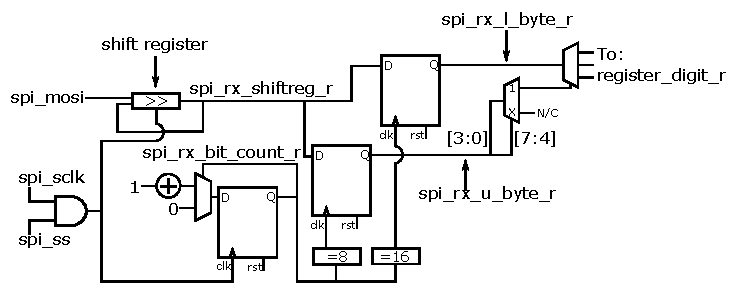
\includegraphics[width=\textwidth]{../rtl_diagrams/display_rx}
	\caption{Simplified RTL diagram of the display's SPI receiver.}
	\label{fig:simple_spi_rx}
\end{figure}

The lower four bits from each of the 8 data registers are concatenated together, forming a 32 bit word. Each of these 4 bit values represents a BCD digit to be displayed, with the rightmost digit controlled by the 4 LSBs, and so on.

The C function that implements allows the programmer to display a value on one of the two subsets of the 7-segment display is listed below. This function borrows heavily from the that which carried out the identical functionality in the previous assignment. Firstly, the value is converted to an array of BCD numbers using the function \lstinline[style={c-style}]|display_value_to_digits|. The array that is filled by this function is then looped over, and the BCD digits are sent to the registers in the display hardware corresponding to their desired positions.
\begin{lstlisting}[style={c-style}]
void display_send_value(uint8_t digit_offset, int16_t value_to_display)
{
	uint8_t inc;
	uint8_t digits[DISPLAY_DIGITS_PER_VAR];
	uint8_t address;
	uint8_t character;
	
	//convert magnitude to specified # of digits
	display_value_to_digits(value_to_display, digits, DISPLAY_DIGITS_PER_VAR); 
	
	for(inc = 0; inc < DISPLAY_DIGITS_PER_VAR; inc++)  //send digits to display
	{   
	    //add increment to offset, +1 due to enable reg @ 0    
		address = digit_offset + inc + 1;
		character = *(digits+inc);
		
		//send character to appropriate digit register
		display_send_write_data(address, character);
	}
}
\end{lstlisting}

\lstinline[style={c-style}]|display_value_to_digits(value_to_display, digits, DISPLAY_DIGITS_PER_VAR)| handles the conversion process from a signed integer, to 4 place array of BCD digits, and is identical to the implementation in the previous assignment, apart from the ability to handle negative numbers. Rather than handling the BCD process differently for negative numbers, the absolute value of the magnitude is taken. To distinguish between positive and negative values, the display has the ability to show a minus sign in the leftmost digit position of that subsection. For positive values, and to avoid the confusion due to a shifting radix at the zero threshold, a blank is shown in this position for positive numbers. The below snippet shows the code implementing this functionality:
\begin{lstlisting}[style={c-style}]
if (value_to_display < 0) 
{
    //reverse 2s complement for negative number & show -
	*(digits+num_digits-1) = DISPLAY_MINUS;
	magnitude = -value_to_display; 
}
else
{
	//top digit is blank for positive values
	*(digits+num_digits-1) = DISPLAY_BLANK; 
	magnitude = value_to_display;
}
\end{lstlisting}




\section*{LED Display}
\subsection*{Design}
The line of LEDs is parallel to the y-axis of the ADXL362, so it is the obvious choice for visualisation on the LEDs. No additional hardware was required to control the LEDs, as they were already connected to the GPIO block provided to us, and accessible over AHB. It was decided that a single LED be lit, representing the acceleration which would act as if it were a ball in a tube, ``rolling'' to either of the ends depending on the force applied. It therefore made sense to set $\pm 1~\si{\gravity}$ as the LEDs at either end, and split the intervening period into a number of evenly spaced acceleration bins.

\subsection*{Implementation}
The y-value to LED lighting was implemented by a single function, as the GPIO interface is simple. \lstinline[style={c-style}]|display_send_led_value(int16_t value_to_display)| handles the conversion from scaled acceleration value to the LED to light. Prior to calling this function, the data from the ADXL has been scaled, such that $1\si~\si{\gravity}$ is represented by $1000$. The first task carried out by this function is the clipping of the acceleration information. Any value with a magnitude greater than $1\si~\si{\gravity}$ is reduced to that level. The signed number representing this value is then shifted so that rather than the centre point lying at zero, the minimum value does. This will make the conversion to an LED index significantly simpler. The shift is carried out by adding the clipping threshold on, as it represents the most negative number in a symmetrical range. As there are no negative values, the result is converted to an unsigned value.
\begin{lstlisting}[style={c-style}]
void display_send_led_value(int16_t value_to_display)
{
	uint16_t led_pos;
	uint16_t us_value_to_display;
	
	const uint16_t scale_to_led_count = (2*DISPLAY_CLIPPING_THRESH)/DISPLAY_NUM_LEDS;
	
	//clip values outside the range
	if(value_to_display > (DISPLAY_CLIPPING_THRESH - 1))
	{
		value_to_display = (DISPLAY_CLIPPING_THRESH - 1);
	}
	else if (value_to_display < -DISPLAY_CLIPPING_THRESH)
	{
		value_to_display = -DISPLAY_CLIPPING_THRESH;
	}
	
	//convert to unsigned value by adding the midpoint on again
	us_value_to_display = (uint16_t) (value_to_display + DISPLAY_CLIPPING_THRESH);
	//light up the lED corresponding to value
	led_pos = us_value_to_display/scale_to_led_count;
	//light up the lED corresponding to value
	pt2GPIO->LED = (1UL << led_pos);
}
\end{lstlisting}

A division is then carried out, which performs the binning process. Integer division will result in truncation, thus assigning the acceleration value to one of the available LED positions.
The result is an integer in the range of $0\rightarrow 15$, as the reduced range of the positive side prevents assignment to a non existent LED at index $16$. The LED itself is set by writing a $1$, shifted to the correct location, to the LED register in the GPIO block provided. This function is declared in \textsc{display.h}.

\section*{Testing}
While testing of Andrew's section of the project was almost entirely based on Verilog test benches in Vivado, this was only possible for the \texttt{Nexys4Display} module. The test bench was written prior to the majority of the module itself, as the hardware was designed starting from the inputs, which meant that the testbench would not change during the process. For the code section of my work, testing was performed by incrementally increasing the complexity of the program, as a test bench is not possible.

\subsection*{Hardware Testing}
The testbench for the display hardware solely tested the SPI hardware, as the \texttt{DisplayInterface} module had previously been tested and confirmed to work at the time of its previous use. Secondly, the \texttt{digit} \& \texttt{segment} outputs of the display hardware are not easily human readable, requiring a complex test bench using \texttt{assert} statements. However, once the SPI hardware had been confirmed to function, a bitstream was generated in which the display registers were initialised to set values to ensure the \texttt{digit} \& \texttt{segment} values still behaved as they had in the past.

As the process of sending data over SPI is a very repetitive process, the test bench exploits Verilog ``tasks'' to simplify the testing process. This task, shown below, takes as input the message to send to the display. The simulated sending of the bits can be done in a loop, which minimises errors due to copy pasting and makes it trivial to send multiple messages.
\begin{lstlisting}[style={verilog-style}]
task send_spi_message;
input [0:15] val_to_send; //indexed in reverse
begin
    clk_spi_x    = 1'b1;
    bits_to_send = 16;
    spi_ss       = 1'b0;
    
    clk_spi_x = #200 1'b0;
    
    for(clock_inc=0;clock_inc<bits_to_send;clock_inc=clock_inc+1)
    begin
        #50  spi_data  = val_to_send[clock_inc];
        #150 clk_spi_x = 1'b1; //send clock high
        if(clock_inc<bits_to_send-1) #200 clk_spi_x = 1'b0; //send clock low
    end
    #10;
    spi_ss = 1'b1;        
end
endtask
\end{lstlisting}
The test bench sends a number of messages, both valid and invalid, to ensure that the correct messages, and only the correct messages, have their payload written into the display registers. Figure \ref{fig:TB} demonstrates the sending of a number of messages, with those containing invalid register addresses or lacking the write command having their value ignored. A failed transaction was also simulated, in which transmission ceased prior its completion. If not correctly designed, subsequent transmissions could appear misaligned, thus having their value ignored unless a hardware reset is performed. This is circumvented in this receiver by clearing the count of bits received once the module slave select returns to the idle position. 
\begin{figure}[h]
	\centering
	\includegraphics[width=\textwidth]{tb}
	\caption{Message Transmission Verilog/Vivado Test Bench.}
	\label{fig:TB}
\end{figure}

\subsection*{Software Testing}
The software was tested in an incremental manner, first decoupling the data collection and display portions of the code to confirm each worked on its own before merging the two sections. As our design featured custom hardware, the tools bundled as part of Keil are unable to simulate the system and tests must be performed using the Nexys 4 board itself.

To test the SPI wrapper for display and the surrounding code, numbers to display were hard coded into the program, to ensure they would appear on the display correctly. This served as test of the display/SPI code, but also of the respective pieces of hardware. Initially this failed to correctly display after the first digit, meaning the count of bits received by the display was likely behaving incorrectly. Examining the signals, and comparing to the combined SPI/Display test bench written by Andrew, it was discovered that the inter-message timing in the test bench had masked a design flaw in the display's receiver. This meant that the bit count came out of reset prematurely, initiating the count and therefore causing byte misalignment.

The benefit of having a second, but simpler, SPI device in the system made the debugging of the code and hardware relating to SPI significantly easier. It was particularly useful that, in contrast to the ADXL, the 7-segment displays served as visual feedback.

With the SPI transmission process complete, the constant value of the first register in the ADXL was used to confirm readback was functioning correctly, printed to the console using the debug channel provided by the serial connection to HyperTerm.

With both portions of the code behaving as expected, they were merged into a single program and tests carried out. From the inspection of the output, it appeared to us that everything was working as intended, however on occasion, writes to the data registers would instead be delivered to the enable register causing the digits to turn off. Examining the SPI lines during transactions on a digital oscilloscope, we discovered that, as our implementation of the SPI master would generate the SPI clock signal as long as the slave select was enabled, a race was created where if the software could not clear slave select quickly enough an extra clock pulse was generated.

After it was pointed out that the system had been over complicated, thus causing this problem, we changed the SPI hardware such that clock pulses would only be generated during the write process, and the ``extra'' pulses required for the readback process generated by sending ``junk'' data bits instead. This removes the potential race condition, and the error causing the display to deactivate itself.

\subsection*{Oscilloscope SPI Screenshots}
Figure \ref{fig:SPI} contains a capture of a write transaction from the process to the display. The message in this case is a write command, address and payload all of 1, and would thus instruct the hardware to draw a 1 on the rightmost digit.
\begin{figure}[h]
	\centering
	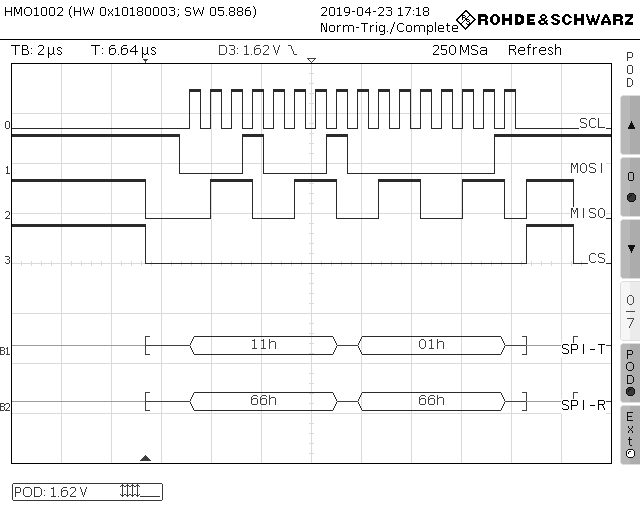
\includegraphics[width=\textwidth]{LAB-03}
	\caption{SPI Write Transaction Between Software and Display Hardware.}
	\label{fig:SPI}
\end{figure}

Figure \ref{fig:SPI_2} contains a capture of the burst read back. This begins with writes of \texttt{0x0B} and \texttt{0x0E} to signal this is a read command beginning at the address of the first register containing the 12 bit data. 6 bytes of \texttt{0xFF} are then transmitted, which the ADXL362 uses to clock out the response onto MISO.
\begin{figure}[h]
	\centering
	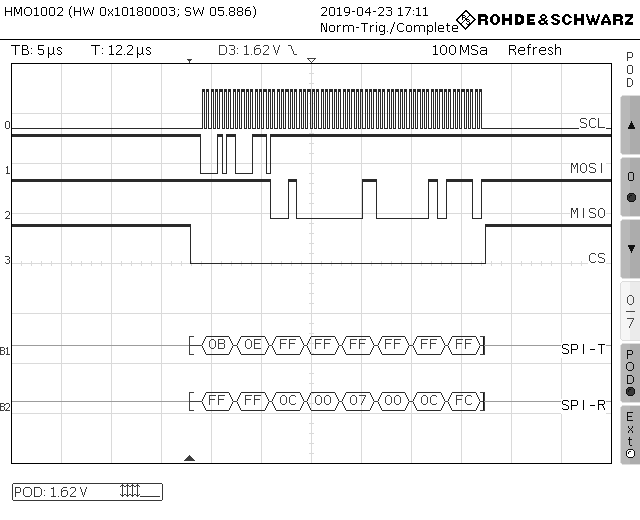
\includegraphics[width=\textwidth]{LAB-02}
	\caption{SPI Burst Read from ADXL362.}
	\label{fig:SPI_2}
\end{figure}
Examining the response bytes, they contain the values $12$, $7$ and $-1012$ for $x$, $y$ and $z$ respectively. This is the expected conditions for the board sitting face up on the bench, as the z-axis runs perpendicular to the plane of the board. $-1024$ would be exactly $1~\si{\gravity}$, so $-1012$ is well within the expected value for this measurement allowing for some measurement inaccuracy.

\section*{System Level Verification}
The correctness of the overall system was checked by angling the board such that the earth's gravitation force was aligned with the measurement direction, and then rotated through $180~\si{\degree}$. The x- and z-axes values were then checked to ensure they lay within the a small margin of $1.00$ and $-1.00$ respectively. Similarly the behaviour of the LEDs corresponding to the y-axes acceleration value was also checked.

\section*{Flaws}
The main flaw with our design was the over-complication of the SPI hardware, although written by Andrew, the behaviour of which was decided between the two of us. I had incorrectly assumed the code would execute quickly enough that the slave select would be cleared before extra pulses would be generated. This was rectified before submission, and converted to the system described above. However, the adjustable size of the transactions remains, which may also represent an over complication of the design.

\section*{Board Configuration}
Figure \ref{fig:brd_cfg} contains an annotated image of the board during operation, as unfortunately a video cannot be embedded into a printable PDF.
\begin{figure}[h]
	\centering
	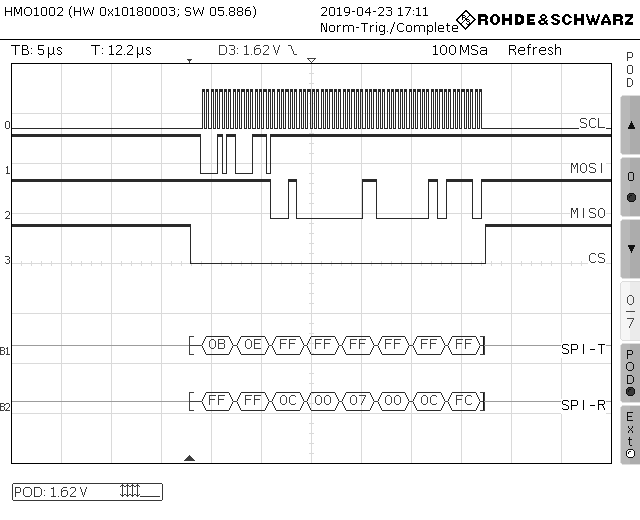
\includegraphics[width=\textwidth]{LAB-02}
	\caption{Nexys 4 Board Configuration.}
	\label{fig:brd_cfg}
\end{figure}

\end{document}